% Took this from CogSci but removed the header, sorry.
%
% Author: Matthew Turner
% Date: 2017-11-23

\documentclass[11pt,letterpaper]{article}

\usepackage{lineno}
\linenumbers
% \usepackage{cogsci}
\usepackage{fullpage}
\usepackage{booktabs}
\usepackage{setspace}
\doublespacing
\usepackage{pslatex}
\usepackage{hyperref}
\usepackage{url}
\usepackage{apacite}
\usepackage{amsmath}
\usepackage{subcaption}
\usepackage[utf8]{inputenc}
\usepackage{pgfplots}
\pgfplotsset{compat=newest}
\usepgfplotslibrary{groupplots}
\usepackage{wrapfig}
\usepackage{bigfoot}
\usepackage[export]{adjustbox}
\setlength\intextsep{0pt}
\usepackage{authblk}



\usepackage{graphicx}

\usepackage{gb4e}  % linguistic examples
\noautomath

\title{Polarization is sensitive to initial opinion extremity and communication noise}

\author[1]{Matthew~A.~Turner}
\author[1]{Paul~E.~Smaldino}

\affil[1]{\footnotesize Cognitive Science Program, University of California, Merced}

\date{}

\begin{document}
\maketitle

\begin{abstract}
  Opinion dynamics in general models how attributes of agents in a population
  change over time. This paper reproduces and extends the investigation of
  \citeA{Flache2011} into how cultural polarization emerges in populations
  connected on a small-world network. Their results do much to shed light
  on what might be the necessary requirements for polarization to occur.
  Importantly, opinions must be measured in a way that allows for negative
  valence of opinion, representing being ``against'' some cultural object.
  Here we add three further considerations we believe are important in 
  modeling when polarization obtains. First, we show that final polarization
  is sensitive to the initial extremity of agent opinions. Second, we quantify
  how robust polarizing dynamics are to noise. 
\end{abstract}

\section{Introduction}


In the most abstract, at any point in time, culture is the state of all
constituent minds each in their individual states. Culture changes when 
individuals change. Individuals change under the influence of other 
individuals. How do individuals change their mental state and how is the
state of culture measured as a whole? There are many possible ways. A popular
metric for characterizing the joint mental state of a population is \emph{polarization}.
Polarization can be measured a multitude of ways \cite{Bramson2016}. The 
concept of polarization has meaning in physics as well---the water molecule
is slightly polarized, for example, giving rise to the van der Waal's force
and high surface tension. In this paper we consider the structural forces that
arise and we call ``polarization'' with respect to agent mental states called
opinions. 

In the model we consider, due to \citeA{Flache2011}, agents' opinions
change based on a weighted difference of their opinions with their neighbors
opinions. Agents are nodes on a network, and relationships are edges of the
network. The edges of this model are weighted and undirected, so each 
connected pair of agents has equal influence over one another, as far as
weights are concerned. A feature of this model is that extremists' opinions
are more entrenched than centrists' opinions, so if an extremist and centrist
are connected, the extremist in a dyad has more \emph{effective} influence 
than a centrist. 

Each agent's mental state is a vector of opinions on a set of cultural features.
The number of cultural features in the model is called the \emph{cultural 
complexity}. 

Social polarization is identified as a precursor to 

One of the first was \cite{Axelrod1997}, where each cultural feature was a 
digit from 1-9, and digits changed. 

\subsection{Summary of Flache and Macy (2011) model}

\section{Methods}
\label{sec:methods}

\section{Results}

\subsection{Initial opinion extremism and polarization}

\citeA{Flache2011} considered the effect of modifying two parameters under their
``Experiment 2.'' This experiment, which is the only one we consider in this
work, experimented with different values of cultural complexity, $K$, and 
different cave sizes. We were curious to understand more about exactly when
polarization emerges, especially with respect to the extremity of opinion
for different cultural complexities. To quantify the affect of extremity of
opinion, we introduced a new parameter $S \in [0, 1]$ that constrains the
extremity of initial opinions. Instead of initial opinions on each
cultural feature being drawn with uniform probability from $[-1, 1]$ they are
instead drawn from $[-S, S]$. 

We performed copmutational experiments to determine the minimum $S$ 
in order for non-zero (greater than 1e-6) polarization to emerge. Clearly if 
$S\leq0.5$ there can be no polarization because all distance are less than 1,
which means all weights will be positive, all
relationships will be friendly, and all agents will be drawn towards some 
consensus point. Our initial experiments (Figure \ref{fig:p_vs_s_for_k})
showed that average polarization was zero for $S < 0.75$ when $K=2$. 
The critical $S$ seems to change for different values of $K$. For example,
average polarization does not increase until $S=0.8$ for $K=3$. For other $K$,
polarization seems to increase to different degrees, with some noise, starting
between $S=0.85$ and $S=0.9$. It appears for $K=3$ that average polarization
decreases from $S=0.95$ to $S=1.0$. There is a large bump in average 
polarization at $S=0.9$ for $K=6$. Is this something real due to some special
configuration for these parameters, or is it noise? (Of course it is not a bug
in our code!)

To better understand the behavior we saw there, we ran a new set of simulations
with 100 trials for each parameter setting, and ran $S$ from 0.75 to 1.0 for
$K=2, 3, 4$ and from 0.85 to 1.0 for $K=5,6$, all with a smaller step size 
of 0.01 (Figure~\ref{fig:zoom_average}). Since the results still appear
noisy, we also plotted median polarization verus $S$ for the different $K$
(Figure~\ref{fig:zoom_median}). The median is still noisy. So, to get even
more detail, we visualized each trial result, and the average, individually
over the $S$ values we tested with 100 trials (Figure~\ref{fig:single_S_K}).
There is indeed a large amount of variation, which seems to increase as $S$
increases.

\begin{figure}[t!]
  \centering
  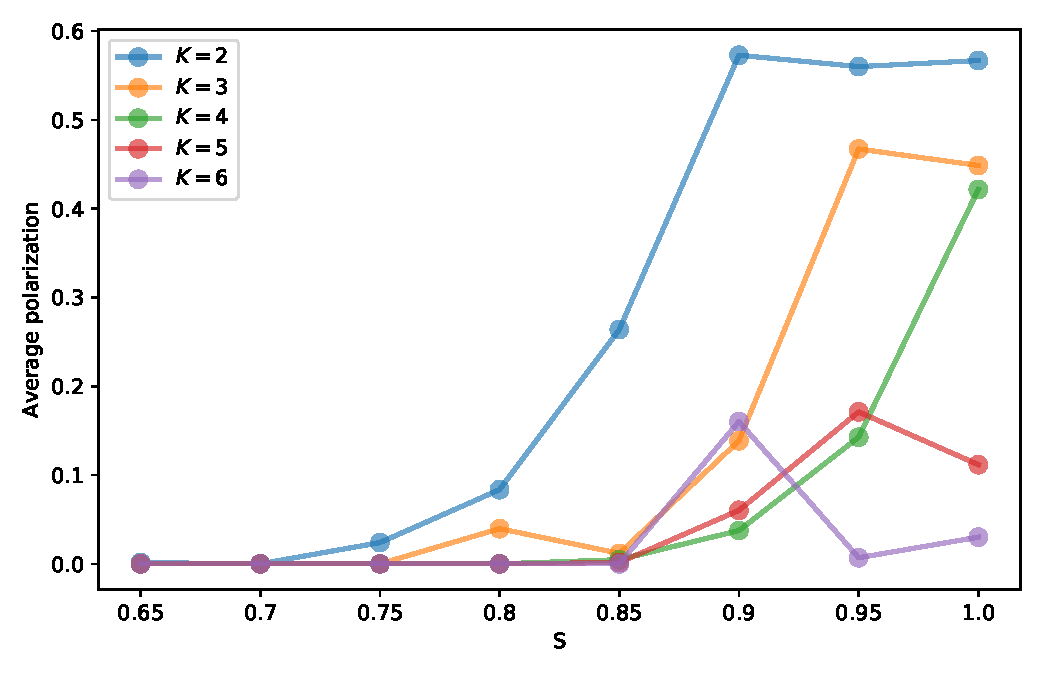
\includegraphics[width=0.75\textwidth]{Figures/P_vs_S_for_K.pdf}
  \caption{
    Average final polarization becomes non-zero then increases as
    the width of the uniform distribution of initial opinions increases.
    The width must be larger and larger as the cultural complexity $K$ 
    increases for the system to achieve non-zero final polarization. This
    condition is identical to the bottom row of each heatmap in 
    Figure \ref{fig:heatmaps}. Each
    data point is the average of fifty trials. Each trial ran over 
    10k timesteps. 
  }
  \label{fig:p_vs_s_for_k}
\end{figure}


\begin{figure}[t!]
  \centering
    \includegraphics[width=0.75\textwidth]{Figures/s_k_zoom_2-6_mean.pdf}
  \caption{Zoom-in on \emph{average} polarization versus $S$ for $K=6$. 
  Different experiment run from Figure~\ref{fig:p_vs_s_for_k}. 
  Same data as in Figure~\ref{fig:zoom_median}.
  Average taken over 100 trials.}
  \label{fig:zoom_average}
\end{figure}

\begin{figure}[h!]
  \centering
    \includegraphics[width=0.75\textwidth]{Figures/s_k_zoom_2-6_median.pdf}
  \caption{Zoom-in on \emph{median} polarization versus $S$ for $K=2,3,4,5,6$. 
    Median polarization for $K=5$ and $K=6$ are both flat at zero; $K=5$ 
    data is obscured by $K=6$.
    Different experiment run from Figure~\ref{fig:p_vs_s_for_k}.
    Same data as in Figure~\ref{fig:zoom_average}.
    Median taken over 100 trials.
  }
  \label{fig:zoom_median}
\end{figure}

% \begin{figure}[t!]
%   \centering
%     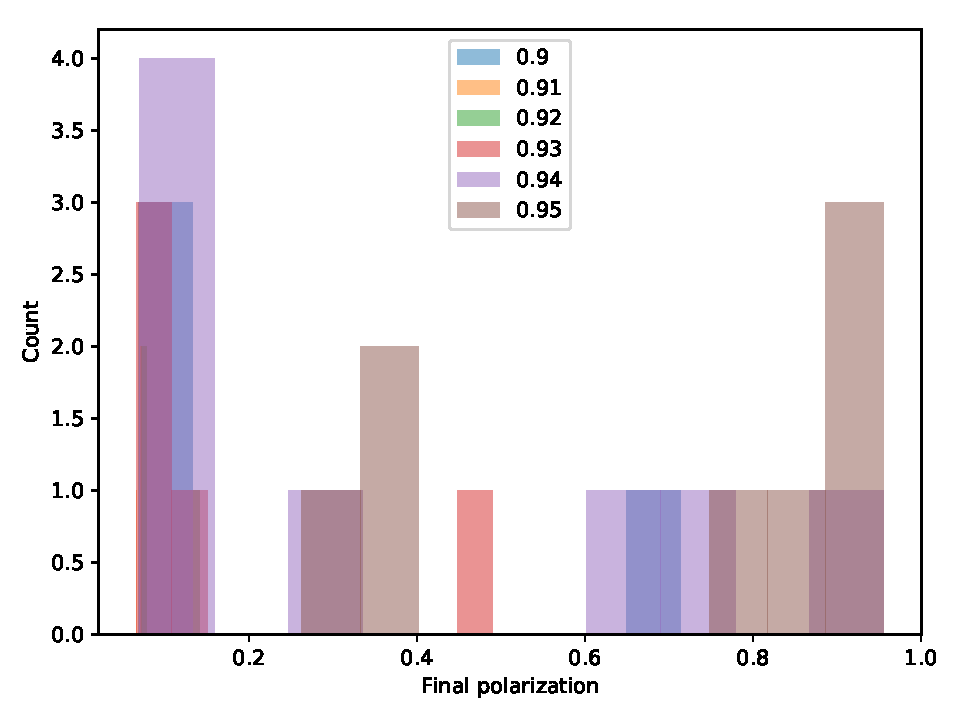
\includegraphics[width=0.75\textwidth]{Figures/p_v_s_k6_histograms.pdf}
%   \caption{Distribution of non-zero final polarization values for $K=6$.
%     Corresponds to the experiment run shown in Figure \ref{fig:zoomK6}.
%   }
%   \label{fig:K6-histograms}
% \end{figure}

\begin{figure}[h!]
  \centering
  \begin{subfigure}[t]{\textwidth}
    \centering
    \includegraphics[width=0.5\textwidth]{Figures/single_S_K=2.pdf}
  \end{subfigure} \\
  \begin{subfigure}[t]{0.49\textwidth}
      \centering
      \includegraphics[width=\textwidth]{Figures/single_S_K=3.pdf}
      % \caption{}
  \end{subfigure}
  ~
  \begin{subfigure}[t]{0.49\textwidth}
      \centering
      \includegraphics[width=\textwidth]{Figures/single_S_K=4.pdf}
      % \caption{}
  \end{subfigure} \\
  \begin{subfigure}[t]{0.49\textwidth}
      \centering
      \includegraphics[width=\textwidth]{Figures/single_S_K=5.pdf}
      % \caption{}
  \end{subfigure}
  ~
  \begin{subfigure}[t]{0.49\textwidth}
      \centering
      \includegraphics[width=\textwidth]{Figures/single_S_K=6.pdf}
      % \caption{}
  \end{subfigure}
  \caption{The average polarization is actually very noisy because 
    final polarizations find a large range of values. Even for $K=6$, there
    are a significant number of trials that end in a non-zero polarization
    state. We need to figure out what causes this. Network configuration?
    Initial conditions? We need to do two tests: hold one or the other 
    constant and vary the other.
  }
  \label{fig:single_S_K}
\end{figure}

\subsection{Sources of single-trial polarization}

This led us to ask two questions. First, how much of this variation was 
present in the original \citeA{Flache2011} paper? Second, what causes
this variability? We begin with the first question. One main result of
\citeA{Flache2011} was that polarization decreases with cultural complexity.
To demonstrate our model is working as theirs is, compare Figure 
\ref{fig:p_vs_K_fm} to Figure 12b of \citeA{Flache2011}---they are identical.
However, when plotting the mean as well as the results of individual trials,
we see that the mean captures some, but not all, of the detail of what's 
happening in terms of opinion dynamics. It is not at all rare for trials to
have final polarizations far from the average 
(Figure~\ref{fig:p_vs_K_single_experiments}). 

\begin{figure}
  \centering
    \includegraphics[width=0.75\textwidth]{Figures/p_vs_K_fm.pdf}
  \caption{Reproduction of Figure 12b of Flache and Macy (2011). The average
    polarization decreases with $K$. However, as shown in subsequent figures,
    this does not mean trials with high polarization never obtain.
  }
  \label{fig:p_vs_K_fm}
\end{figure}


\begin{figure}[h!]
  \centering
    \begin{subfigure}[t]{\textwidth}
      \centering
      \includegraphics[width=.65\textwidth]{Figures/connected-caveman-over-K.pdf}
      \caption{Final polarizations for the non-random connected caveman graph.}
      \label{fig:connected-caveman-trials}
    \end{subfigure}
    \begin{subfigure}[t]{\textwidth}
      \centering
      \includegraphics[width=.65\textwidth]{Figures/random-shortrange-over-K.pdf}
      \caption{Final polarizations for the non-random connected caveman graph.}
      \label{fig:random-shortrange-trials}
    \end{subfigure}
    \begin{subfigure}[t]{\textwidth}
      \centering
      \includegraphics[width=.65\textwidth]{Figures/random-anyrange-over-K.pdf}
      \caption{}
      \label{fig:random-anyrange-trials}
    \end{subfigure}
  \caption{Even in the non-random connected caveman structure, there is 
    variation in the final polarization for different values of $K$. Highly
    polarized final states may obtain. 100 trials are shown and comprise the
    average. The circle shows the result for one trial of the configuration
    reused to make Figure~\ref{fig:single-ic-histogram}.
  }
  \label{fig:single-experiments-over-k}
\end{figure}

The answer to our first question is, yes, there is much variation in the 
results from \citeA{Flache2011}. We turn to our second question, where does
this variation come from? It seems there are two sources: the specific
initial opinions that agents draw from the uniform distribution and the
update path. As (WILL BE) explained in the introduction, the \citeA{Flache2011}
an iteration is defined as $N$ updates of either a weight or an edge. 
By ``update path,'' we mean which edges or weights are updated in what order. 

First, to see what effect the exact initial distribution has on the final 
polarization we regressed final polarization against initial polarization for
$K=2$ for the non-random connected caveman graph 
(Figure~\ref{fig:final-initial-pol-regplot}, whose final polarizations are 
plotted in the $K=2$ column of Figure~\ref{fig:connected-caveman-trials}.
While there is a trend, there is still much noise with final polarizations
far above and below the regression line. 

To evaluate the path dependence, we ran another 100 trials using the initial
conditions from the $K=2$, connected caveman trial
with the maximum final polarization of 0.86. The distribution of outcomes was
skewed towards polarizations higher than the mean for connected caveman, $K=2$,
which was .41 (Figure~\ref{fig:highpol-histogram}). However, there are many,
though a minority, of trials that end \emph{below} that mean. This seems to
suggest that update path has a large impact on the final polarization of a
given trial. However, initial conditions can bias the final polarization. 

Why is this? Consider the space of all update paths. 
There are ($N_{iter} \times N_{agents} \times N_{weights}$?) of these.
I hypothesize this is because larger initial polarizations means a larger
fraction of these paths are polarizing. This may well be related to the 
concept of signed graphs: graphs where one can perfectly separate the graph
into two graphs where all agents are friendly with each other, i.e. 
$w_{ij} > 0$ for all agents $i,j$ \cite{Altafini2012}. There are measures of
signedness, and I have a feeling that signedness tracks with polarization.
That is, as the iterations progress, we could plot signedness as well as 
polarization, and when signedness breaks different thresholds, higher levels of
polarization become inevitable.

\begin{figure}[h!]
  \centering
    \includegraphics[width=.75\textwidth]{Figures/final-initial-pol-regplot.pdf}
  \caption{Final and initial polarizations shown for $K=2$ with the connected 
    caveman network. Final polarizations are same as in the $K=2$ column of 
    Figure~\ref{fig:final-initial-pol-regplot}}
  \label{fig:average-trial-caveman-over-k}
\end{figure}

\begin{figure}[h!]
  \centering
    \includegraphics[width=.75\textwidth]{Figures/caveman-highpol-histogram-10k-its.pdf}
  \caption{Distribution of final polarizations at iteration 10000
  starting from initial conditions
  of the connected caveman trial with the largest final polarization with $K=2$.
  The distribution is skewed towards final polarizations considerably larger
  than the mean polarization of 0.41 for the connected caveman experiment
  with $K=2$. 
  }
  \label{fig:highpol-histogram}
\end{figure}



% \subsection{Communication noise and polarization}

% \begin{figure}[t!]
%   \centering
%       \begin{subfigure}[t]{0.49\textwidth}
%           \centering
%           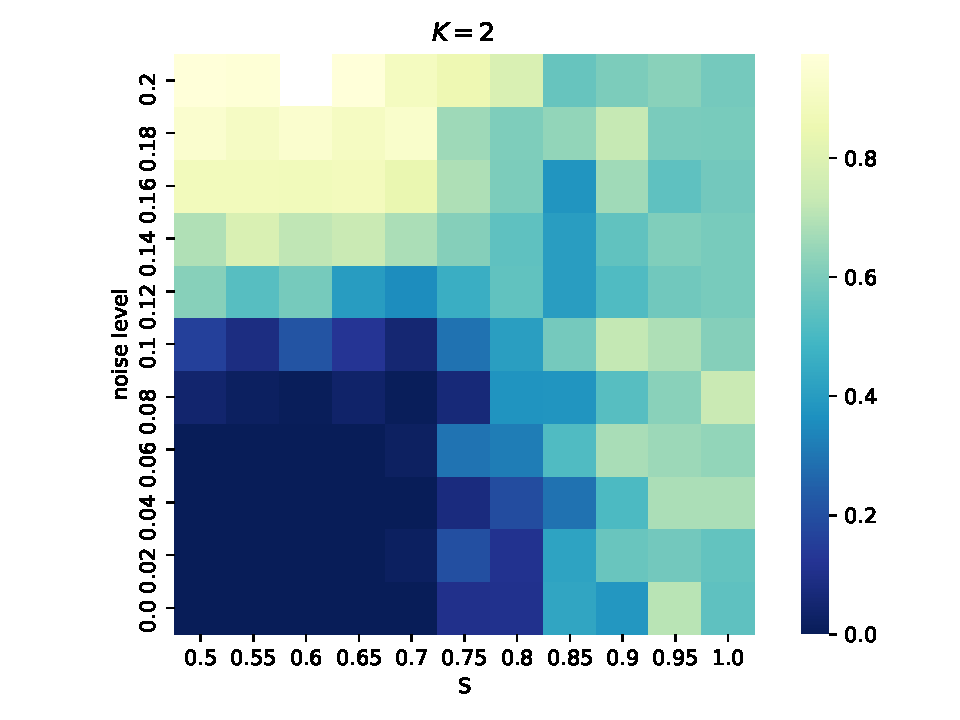
\includegraphics[width=\textwidth]{Figures/p_v_noise_k=2.pdf}
%           \caption{}
%       \end{subfigure}
%       ~
%       \begin{subfigure}[t]{0.49\textwidth}
%           \centering
%           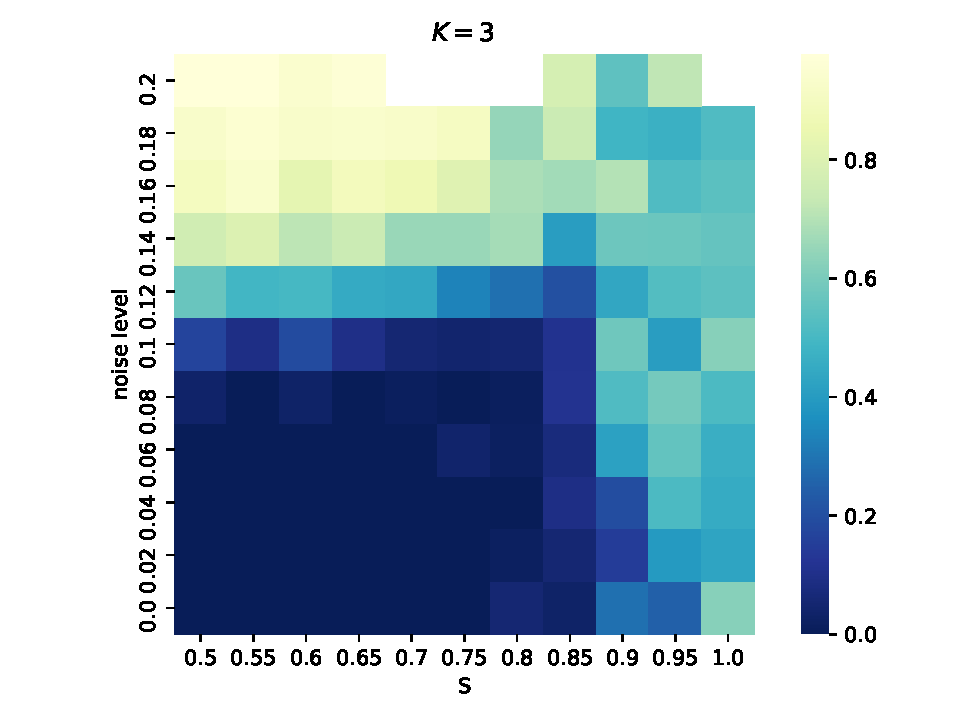
\includegraphics[width=\textwidth]{Figures/p_v_noise_k=3.pdf}
%           \caption{}
%       \end{subfigure} \\
%       \begin{subfigure}[t]{0.49\textwidth}
%           \centering
%           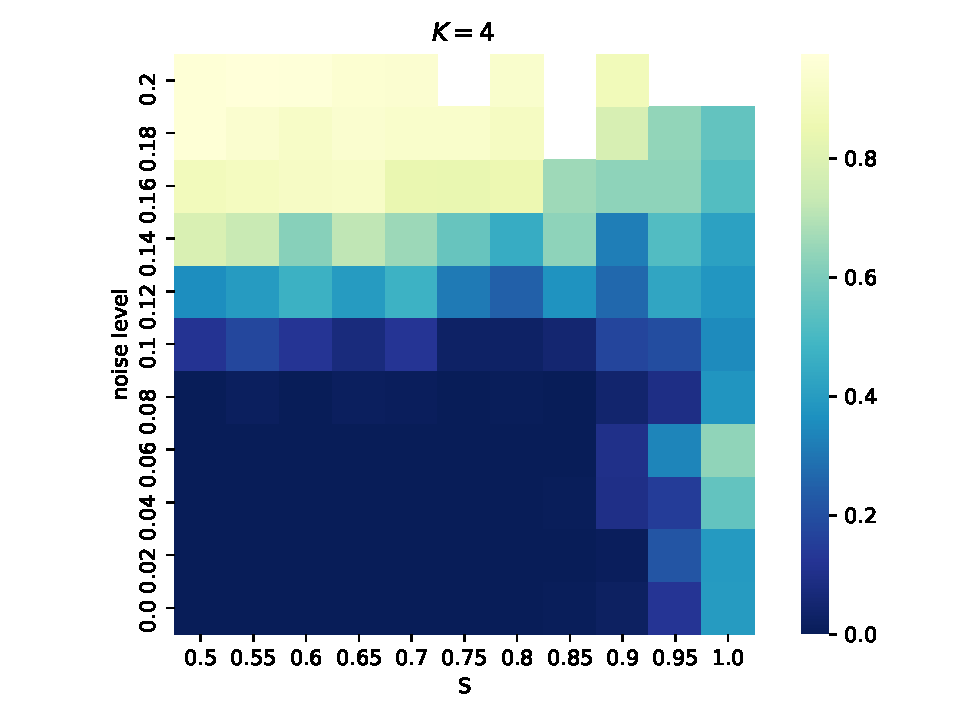
\includegraphics[width=\textwidth]{Figures/p_v_noise_k=4.pdf}
%           \caption{}
%       \end{subfigure}
%       ~
%       \begin{subfigure}[t]{0.49\textwidth}
%           \centering
%           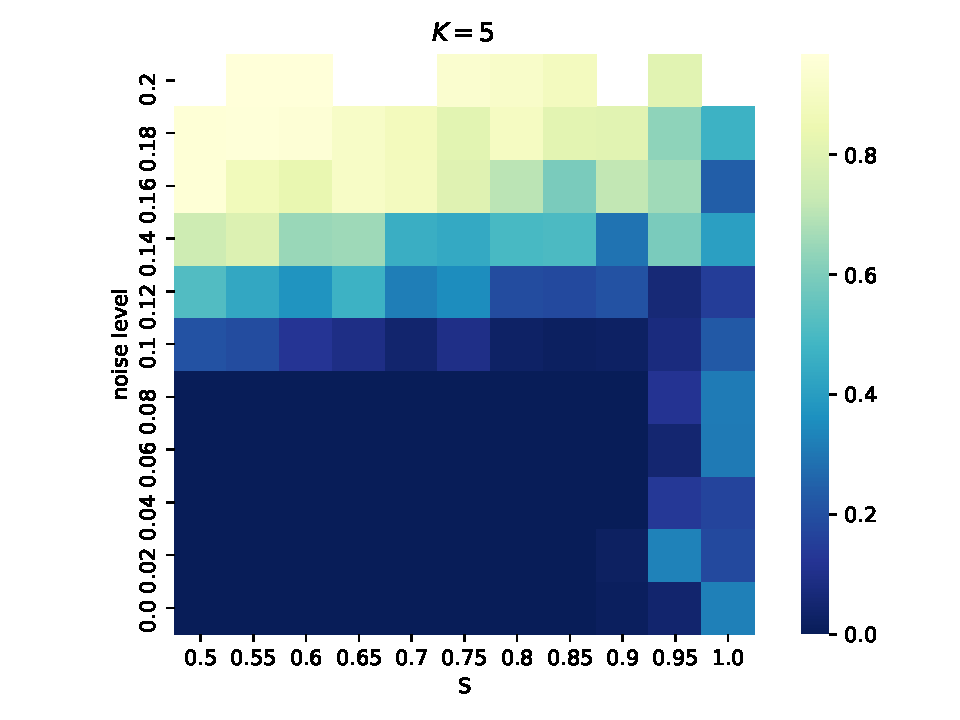
\includegraphics[width=\textwidth]{Figures/p_v_noise_k=5.pdf}
%           \caption{}
%       \end{subfigure} \\
%   \caption{Final average polarization varies with both the width of the
%     uniform distribution of initial opinion magnitudes and the noise level in
%     the opinion updates. Noisy opinion updates can perturb the system away from
%     situations where homogeneity of opinion would otherwise obtain. $K=2,3,4,5$
%     are shown. The value in each square of the heatmap is the average of
%     fifty trials. Each trial ran over 10k timesteps.
%   }
%   \label{fig:heatmaps}
% \end{figure}



\clearpage

\bibliographystyle{apacite}

\setlength{\bibleftmargin}{.125in}
\setlength{\bibindent}{-\bibleftmargin}

\bibliography{/Users/mt/workspace/papers/library.bib}

\end{document}
